% Chapter Template

\chapter{Introduction} % Main chapter title

\label{Chapter2} % Change X to a consecutive number; for referencing this chapter elsewhere, use \ref{ChapterX}

\lhead{Chapter 1. \emph{Introduction}} % Change X to a consecutive number; this is for the header on each page - perhaps a shortened title

%----------------------------------------------------------------------------------------
%	SECTION 1
%----------------------------------------------------------------------------------------

\section{Motivation}

Scramjet engines are on the forefront of supersonic transportation development because of their simplicity and promising outlook for steady and reliable supersonic combustion. These engines differ from typical subsonic jet engines, as scramjets have no moving parts and simply rely on shock waves produced at these supersonic speeds to compress the intake air and provide the means for ignition.

One challenge facing the production of these engines is producing steady combustion. Much like keeping a match lit in a hurricane, keeping a flame stabilized at supersonic speeds is difficult. One proposed method of flame stabilization is a rectangular cavity. These cavities, like the cavity shown in Figure \ref{CavDiagram}, are able provide a re-circulation zone with high temperatures and combustion radicals for strong combustion to occur. Many experimental studies have tested the flame-holding abilities of cavities in strong combustion cases \cite{ben2000experimental,ben2001cavity,do2009plasma,yilmaz2013investigation}. Strong combustion occurs when the fuel-air mixture is optimized for efficient fuel burning. The mixture in strong combustion cases occur in proper stoichiometric proportions. These studies focused on cavity dimensions and how the length to depth ratio, L/D, affects key ignition and flame holding characteristics, such as stagnation pressure, stagnation temperature, fuel air mixture, and residence time. Ben-Yakar concluded that with L/D ratios between 4 and 10, strong combustion can be sustained in these cavities for total enthalpy flight conditions of Mach 8, 10, and 13\cite{ben2001cavity}. Also noted in several investigations is the presence of strong acoustic waves\cite{unalmis2004cavity,heller1996letter,williams2007supersonic, mcgregor1970drag,luo2011drag, sato1999advanced}. 

Similar to blowing air over an empty bottle to create a tone, the freestream air traveling over and interacting with these cavities produces acoustic waves. In these cavities, a shear layer develops between the high speed freestream and the slower, re-circulating air in the cavity. As the shear layer travels downstream, it begins to drop. By the time the shear layer reaches the downstream wall of the cavity, it has lowered to a point where the interaction of the shear layer with the downstream wall of the cavity produces strong pressure waves, which propagate upstream, ultimately resonating within the cavity. 

Other experimental studies have investigated the acoustic properties of these cavities \cite{unalmis2004cavity,heller1996letter,williams2007supersonic, mcgregor1970drag,luo2011drag, sato1999advanced}. These investigations concluded that the acoustic waves generated by supersonic cavities produce several undesirable effects. One effect, investigated by McGregor is the induced drag associated with rectangular cavities. The effect of pressure waves within these cavities can increase the drag by as much as 250\% \cite{mcgregor1970drag}. These acoustic waves can also have an adverse effect on equipment and the crew. At low frequencies, the resonating acoustic waves can cause structural damage to the engine. At high frequencies, these waves can cause uneasiness in crew members \cite{mcgregor1970drag}.

Conclusions drawn from these investigations have led to the desire to suppress these acoustic waves. Suppressing these waves would reduce drag on the engine and cause less damage to the engine or the crew. However, these acoustic waves could have the potential to assist in combustion when conditions for weak combustion are present. Weak combustion, as is studied in this investigation, is at lean fuel air mixture conditions. Sato et al.\cite{sato1999advanced} investigated the enhancement of mixing due to acoustic waves. They concluded that mixing was enhanced by these acoustic waves and the rate of enhancement was controlled by the cavity's shape. However, the investigations performed by Sato et al. did not include the cavity as a flame-holder. The cavity was only used to produce the mixing enhancing acoustic waves. 

Few, if any, experimental studies have investigated the acoustic properties of these cavities as they assist in mixing and the enhancement of combustion at lean conditions. This investigation is broken into three parts, which together will provide a clear interpretation of a cavity's suitability as an effective flame holder during weak combustion conditions. The first part of the investigation isolates the acoustic properties of the cavities. The frequency of a cavity can be estimated using an empirical equation derived by Heller and Delfs \cite{heller1996letter}, as shown in Equation \ref{eq:freq}. This equation is estimated to be able to predict the frequency within the cavity $\pm$10\%\cite{heller1996letter}.

\begin{equation}
f_m = \frac{m-\alpha}{\{M_{\infty}/\sqrt{1+[(\gamma_{\infty}-1)/2]M_{\infty}^2}+1/k\}} \cdot \frac{U_\infty}{L}
\label{eq:freq}
\end{equation}


%-----------------------------------
%	SUBSECTION 1
%-----------------------------------
\subsection{Subsection 1}

Nunc posuere quam at lectus tristique eu ultrices augue venenatis. Vestibulum ante ipsum primis in faucibus orci luctus et ultrices posuere cubilia Curae; Aliquam erat volutpat. Vivamus sodales tortor eget quam adipiscing in vulputate ante ullamcorper. Sed eros ante, lacinia et sollicitudin et, aliquam sit amet augue. In hac habitasse platea dictumst.

%-----------------------------------
%	SUBSECTION 2
%-----------------------------------

\subsection{Subsection 2}
Morbi rutrum odio eget arcu adipiscing sodales. Aenean et purus a est pulvinar pellentesque. Cras in elit neque, quis varius elit. Phasellus fringilla, nibh eu tempus venenatis, dolor elit posuere quam, quis adipiscing urna leo nec orci. Sed nec nulla auctor odio aliquet consequat. Ut nec nulla in ante ullamcorper aliquam at sed dolor. Phasellus fermentum magna in augue gravida cursus. Cras sed pretium lorem. Pellentesque eget ornare odio. Proin accumsan, massa viverra cursus pharetra, ipsum nisi lobortis velit, a malesuada dolor lorem eu neque.

%----------------------------------------------------------------------------------------
%	SECTION 2
%----------------------------------------------------------------------------------------

\section{Main Section 2}

Sed ullamcorper quam eu nisl interdum at interdum enim egestas. Aliquam placerat justo sed lectus lobortis ut porta nisl porttitor. Vestibulum mi dolor, lacinia molestie gravida at, tempus vitae ligula. Donec eget quam sapien, in viverra eros. Donec pellentesque justo a massa fringilla non vestibulum metus vestibulum. Vestibulum in orci quis felis tempor lacinia. Vivamus ornare ultrices facilisis. Ut hendrerit volutpat vulputate. Morbi condimentum venenatis augue, id porta ipsum vulputate in. Curabitur luctus tempus justo. Vestibulum risus lectus, adipiscing nec condimentum quis, condimentum nec nisl. Aliquam dictum sagittis velit sed iaculis. Morbi tristique augue sit amet nulla pulvinar id facilisis ligula mollis. Nam elit libero, tincidunt ut aliquam at, molestie in quam. Aenean rhoncus vehicula hendrerit.

%-------------------------------------------------------
%    FIGURES
%------------------------------------------------------

\begin{figure}
\centering
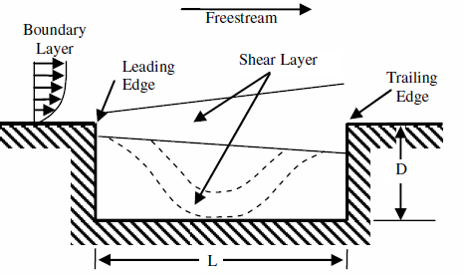
\includegraphics[height=3in]{Figures/CavityDiagram.png}
\caption[Diagram of typical cavity]{Typical hypersonic cavity schematic \cite{lazar2008control}.}
\end{figure}